\documentclass[11pt]{article}
\usepackage{enumitem}
\usepackage{float}
\usepackage[margin=1in]{geometry}
\usepackage{graphicx}
\usepackage[space]{grffile}
\usepackage{adjustbox}
\usepackage{amsmath}
\usepackage{amsthm}
\usepackage{amssymb}
\usepackage{fullpage}
\usepackage{fancyhdr}
\usepackage{xparse}
\usepackage[makeroom]{cancel}
\newcommand{\cnum}{CM146}
\newcommand{\ced}{Fall 2018}
\newcommand{\ctitle}[3]{\title{\vspace{-0.5in}\cnum, \ced\\Problem Set #1: #2}}
\newcommand{\solution}[1]{{{\color{blue}{\bf Solution:} {#1}}}}
\NewDocumentCommand{\texcod}{mm}{%
	\texttt{\textcolor{#1}{#2}}%
}
\usepackage[usenames,dvipsnames,svgnames,table,hyperref]{xcolor}
\usepackage{listings}
\usepackage{color} %red, green, blue, yellow, cyan, magenta, black, white
\definecolor{mygreen}{RGB}{28,172,0} % color values Red, Green, Blue
\definecolor{mylilas}{RGB}{170,55,241}

\renewcommand*{\theenumi}{\alph{enumi}}
\renewcommand*\labelenumi{(\theenumi)}
\renewcommand*{\theenumii}{\roman{enumii}}
\renewcommand*\labelenumii{\theenumii.}

\author{Zheng Wang (404855295)}
\date{\today}
\title{MATH 151B Homework 2}

\begin{document}
	
\lstset{language=Matlab,%
	basicstyle=\footnotesize,
	breaklines=true,%
	morekeywords={matlab2tikz},
	keywordstyle=\color{blue},%
	morekeywords=[2]{1}, keywordstyle=[2]{\color{black}},
	identifierstyle=\color{black},%
	stringstyle=\color{mylilas},
	commentstyle=\color{mygreen},%
	showstringspaces=false,%without this there will be a symbol in the places where there is a space
	numbers=left,%
	numberstyle={\tiny \color{black}},% size of the numbers
	numbersep=9pt, % this defines how far the numbers are from the text
	emph=[1]{for,end,break},emphstyle=[1]\color{red}, %some words to emphasise
	%emph=[2]{word1,word2}, emphstyle=[2]{style},    
}

\maketitle
\section*{Question 1}
\begin{itemize}
	\item [(a)]
	First of all, we derive the term $ T^{(4)}(t_i,w_i) $ as the following:
	\begin{equation*}
	\begin{aligned}
	T^{(4)}(t_i, w_i) &= f(t_i,w_i) + \frac{h}{2}f'(t_i,w_i) + \frac{h^2}{6}f''(t_i.w_i) + \frac{h^3}{24}f'''(t_i,w_i)\\
	&=(t_i^2 - 1) + \frac{h}{2}(2t_i) + \frac{h^2}{6}\cdot 2 + \frac{h^3}{24}\cdot 0\\
	&=t_i^2 + ht_i + \frac{h^2}{3} - 1
	\end{aligned}
	\end{equation*}
	Thus, the Taylor Method of order 4 gives us the following:
	\[\begin{cases}
	w_0 = 0\\
	w_{i+1} = w_i + h(t_i^2 + ht_i + \frac{h^2}{3} - 1)\quad \text{for each } i = 0,\ 1,...,\ N-1
	\end{cases} \]
	\item [(b)]
	Using $ h = 1 $, we have the following from the Taylor Method of order 4:
	\begin{equation*}
	\begin{aligned}
	y(1) = w_1 &= y(0) + h\cdot(t_0^2 + ht_0 + \frac{h^2}{3} - 1)\\
	&= 0 + 1\times(0^2 + 1\times0 + \frac{1^2}{3} - 1)\\
	&= \boxed{-\frac{2}{3}}
	\end{aligned}
	\end{equation*}
	To find the exact solution, we have the following process:
	\[ \frac{dy}{dt} = t^2 - 1 \quad\Longrightarrow\quad \int dy = \int t^2 - 1\ dt \quad \Longrightarrow\quad y = \frac{t^3}{3} -t + C\]
	Now, since $ y(0) = 0 $, we have $ C= 0  $. Thus, the solution to the IVP is $ \displaystyle\boxed{y = \frac{t^3}{3} -t}$. \\
	So, $ \displaystyle y(1) = \frac{1}{3} - 1 = \boxed{-\frac{2}{3}} $, and the error is $ 0 $. The error is zero because the original funtion $ y(t) $ is a polynomial of degree $ 3 $. Thus, the corresponding local truncation error when we use Talyor's method of degree 4 is $\displaystyle \tau_1(h) =  \frac{h^5}{5!}y^{(5)}(\xi_i) = 0 $, where $ \xi_i\in (0,1) $. So, the result is exact. \pagebreak
\end{itemize}
\section*{Question 2}
\begin{itemize}
	\item [(a)]
	Using the multivariable version of Taylor Method, we have the following ($ R_1$ is the remainder term): 
	\begin{equation*}
	\begin{aligned}
	&\quad\ a_1f(t,y) + a_2f(t+\alpha, y + \beta f(t,y))\\ 
	&= a_1 f(t,y) + a_2[f(t,y) + \alpha\cdot f_t(t,y) + \beta\cdot f(t,y) \cdot f_y(t,y) + R_1(t+\alpha, y + \beta f(t,y)) ]\\
	&= (a_1+a_2)f(t,y) + a_2\alpha \cdot f_t(t,y) + a_2\beta\cdot f(t,y) \cdot f_y(t,y) + a_2R_1\\
	\end{aligned}
	\end{equation*}
	When align the coefficient, we leave $ R_1 $ out and use:\\ $  a_1f(t,y) + a_2f(t+\alpha, y + \beta f(t,y)) \approx (a_1+a_2)f(t,y) + a_2\alpha \cdot f_t(t,y) + a_2\beta\cdot f(t,y) \cdot f_y(t,y) $\\
	By align the coefficient, we have the following:
	\[ \begin{cases}
	a_1+a_2 = 1\\
	a_2\cdot \alpha = \frac{h}{2}\\
	a_2\cdot \beta = \frac{h}{2}
	\end{cases} \]
	Thus, one way of choosing the coefficient is:
	\[ \begin{cases}
	a_1 = 0\\
	a_2 = 1\\
	\alpha = \frac{h}{2}\\
	\beta = \frac{h}{2}
	\end{cases} \]
	
	\item [(b)]
	By setting $ a_1 = \frac{1}{2} $, we then have the following solution:
	\[ \begin{cases}
	a_1 = \frac{1}{2}\\
	a_2 = \frac{1}{2}\\
	\alpha = h\\
	\beta = h
	\end{cases} \]
	Then, the approximation of $ T^{(2)}(t,y) $ break downs to $ \frac{1}{2}f(t,y) + \frac{1}{2}f(t+h,y+hf(t,y)) $. Thus, the modified Euler Method is given as below:
	\[ \begin{cases}
	w_0 = \alpha\\
	w_{i+1} = w_i + \frac{h}{2}[f(t_i,w_i) + f(t_{i+1},w_i+hf(t_i,w_i))]\quad\text{for each } i = 0,1,...,N-1
	\end{cases} \]\pagebreak
	
	\item [(c)]
	By the formula of local truncation error of difference method, we have the following:
	\begin{equation*}
	\begin{aligned}
	\tau_{i+1}(h) &= \frac{y_{i+1}-y_i}{h} - \frac{1}{2}[f(t_i,y_i) + f(t_{i+1},y_i+hf(t_i,y_i))]\\
	&=\frac{ \cancel{y(t_i)} + h\cancel{y'(t_i) }+ \cancel{\frac{h^2}{2}y''(t_i)} + \frac{h^3}{6}y'''(t_i) + \mathcal{O}(h^4)- \cancel{y(t_i)}}{h}\\
	&\quad-\frac{1}{2}[\cancel{f(t_i,y_i) + f(t_i,y_i)} + \cancel{h\frac{\partial f}{\partial t}(t_i,y_i) + hf(t_i,y_i)\frac{\partial f}{\partial y}(t_i,y_i)}\\
	&\quad+\frac{h^2}{2}\frac{\partial^2 f}{\partial t^2}(t_i,y_i) + \frac{h^2f(t_i,y_i)^2}{2}\frac{\partial^2 f}{\partial y^2}(t_i,y_i)+h^2f(t_i,y_i)\frac{\partial^2 f}{\partial t\partial y}(t_i,y_i) + \mathcal{O}(h^3) ]\\
	&= \frac{h^2}{6} \left(\frac{\partial^2 f}{\partial t^2}(t_i,y_i) + \frac{\partial^2 f}{\partial y^2}(t_i,y_i)f(t_i,y_i)^2 + 2f(t_i,y_i)\frac{\partial^2 f}{\partial t\partial y}(t_i,y_i) + \frac{\partial f}{\partial y}(t_i,y_i)f'(t_i,y_i) \right)\\
	&\quad- \frac{1}{2}\left( \frac{h^2}{2}\frac{\partial^2 f}{\partial t^2}(t_i,y_i) + \frac{h^2f(t_i,y_i)^2}{2}\frac{\partial^2 f}{\partial y^2}(t_i,y_i)+h^2f(t_i,y_i)\frac{\partial^2 f}{\partial t\partial y}(t_i,y_i) \right) + \mathcal{O}(h^3)\\
	&=\frac{h^2}{6}\frac{\partial f}{\partial y}(t_i,y_i)f'(t_i,y_i) - \frac{1}{12}h^2\left( \frac{\partial^2 f}{\partial t^2}(t_i,y_i) + \frac{\partial^2 f}{\partial y^2}(t_i,y_i)f(t_i,y_i)^2 + 2f(t_i,y_i)\frac{\partial^2 f}{\partial t\partial y}(t_i,y_i)  \right)\\
	&\quad+ \mathcal{O}(h^3)
	\end{aligned}
	\end{equation*}
	By assuming that all partial derivatives are bounded, we have $ \tau_{i+1}(h) \le Mh^2 $\\
	Thus, the error is of order 2 (i.e. $ \mathcal{O}(h^2) $).
	\item [(d)]
	At the first step, we have $ w_0 = 0 $.\\
	Secondly, we have $\displaystyle y(0.5) = w_1 = 0 + \frac{0.5}{2}(f(0,0) + f(0.5,0.5\times f(0,0) ))  = -\frac{7}{16}$.\\
	Finally, we have $\displaystyle y(1) = -\frac{7}{16} + \frac{0.5}{2}(f(0.5,-\frac{7}{16}) + f(1,0.5\times f(0.5,-\frac{7}{16})) = \boxed{-\frac{5}{8}}$.
	
\end{itemize}

\section*{Question 4}
\begin{itemize}
	\item [(a)]
	The Heun’s Method is implemented with the function \texcod{blue}{heun}:
	\lstinputlisting{heuns.m}
	The output from the console is $ \boxed{2.7177} $, which is approximately the correct result of the $ y(1) = e $.
	\begin{verbatim}
	>> heuns
	    2.7177
	\end{verbatim}
	
	\item [(b)]
	I used following IVP for generating this plot:
	\[ y'(t) = y^2e^{-t},\ 0\le t \le 1,\ y(0)=1 \]
	The plot I obtained by runing Heun's Method, Modified Euler's Method, and Euler's Method are given below:\\
	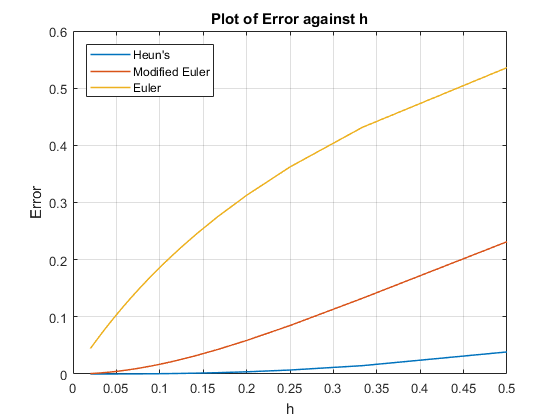
\includegraphics{error.png}\\
	We can see that the error of Euler's method is approximately linear, and it is the largest among the three method. The error of Modified Euler's method is smaller than Euler's method, and the increasing trending is approximately quadratic. Finally, the error of the Heun's Method is the smallest among the three method, and the increasing tending of error as $ h $ increase is approximatly cubic. Thus, this verifies that error of Euler's Method is $ \mathcal{O}(h) $, the error of Modified Euler's Method is $ \mathcal{O}(h^2) $, and the error of Heun's Method is $ \mathcal{O}(h^3) $.\\\\\\\\
	The code for generating the plot is given below:\\
	\lstinputlisting{order.m}
	
\end{itemize}


\end{document}